\newpage

\section{The ABCD' Technique}
\label{app:abcdprime}

We have developed a novel technique, based on the ABCD technique which we perform
in the plane of $y$ vs. \Ht, which allows us to estimate the background in a signal
region defined in the \met\ vs. \Ht\ plane. We refer to this as the ABCD' technique.

First, we extract the $y$ and \Ht\ distributions $f(y)$ and $g(H_T)$ from data, using 
events from control regions which we expect to be dominated by background. Under the assumption
that $y$ and \Ht\ are weakly-correlated (the same assumption which allows the use of
the ABCD technique), we can predict the distribution of events in the $y$ vs. \Ht\ plane as:

\begin{equation}
\frac{\partial^2 N}{\partial y \partial H_T} = f(y)g(H_T)
\end{equation}

Once the distribution of events in the $y$ vs. \Ht\ plane is known, the number of events
falling in any region of this plane can be deduced. In particular, we can deduce the
number of events falling in a region defined by requirements on \met\ and \Ht.


\begin{figure}[tbh]
\begin{center}
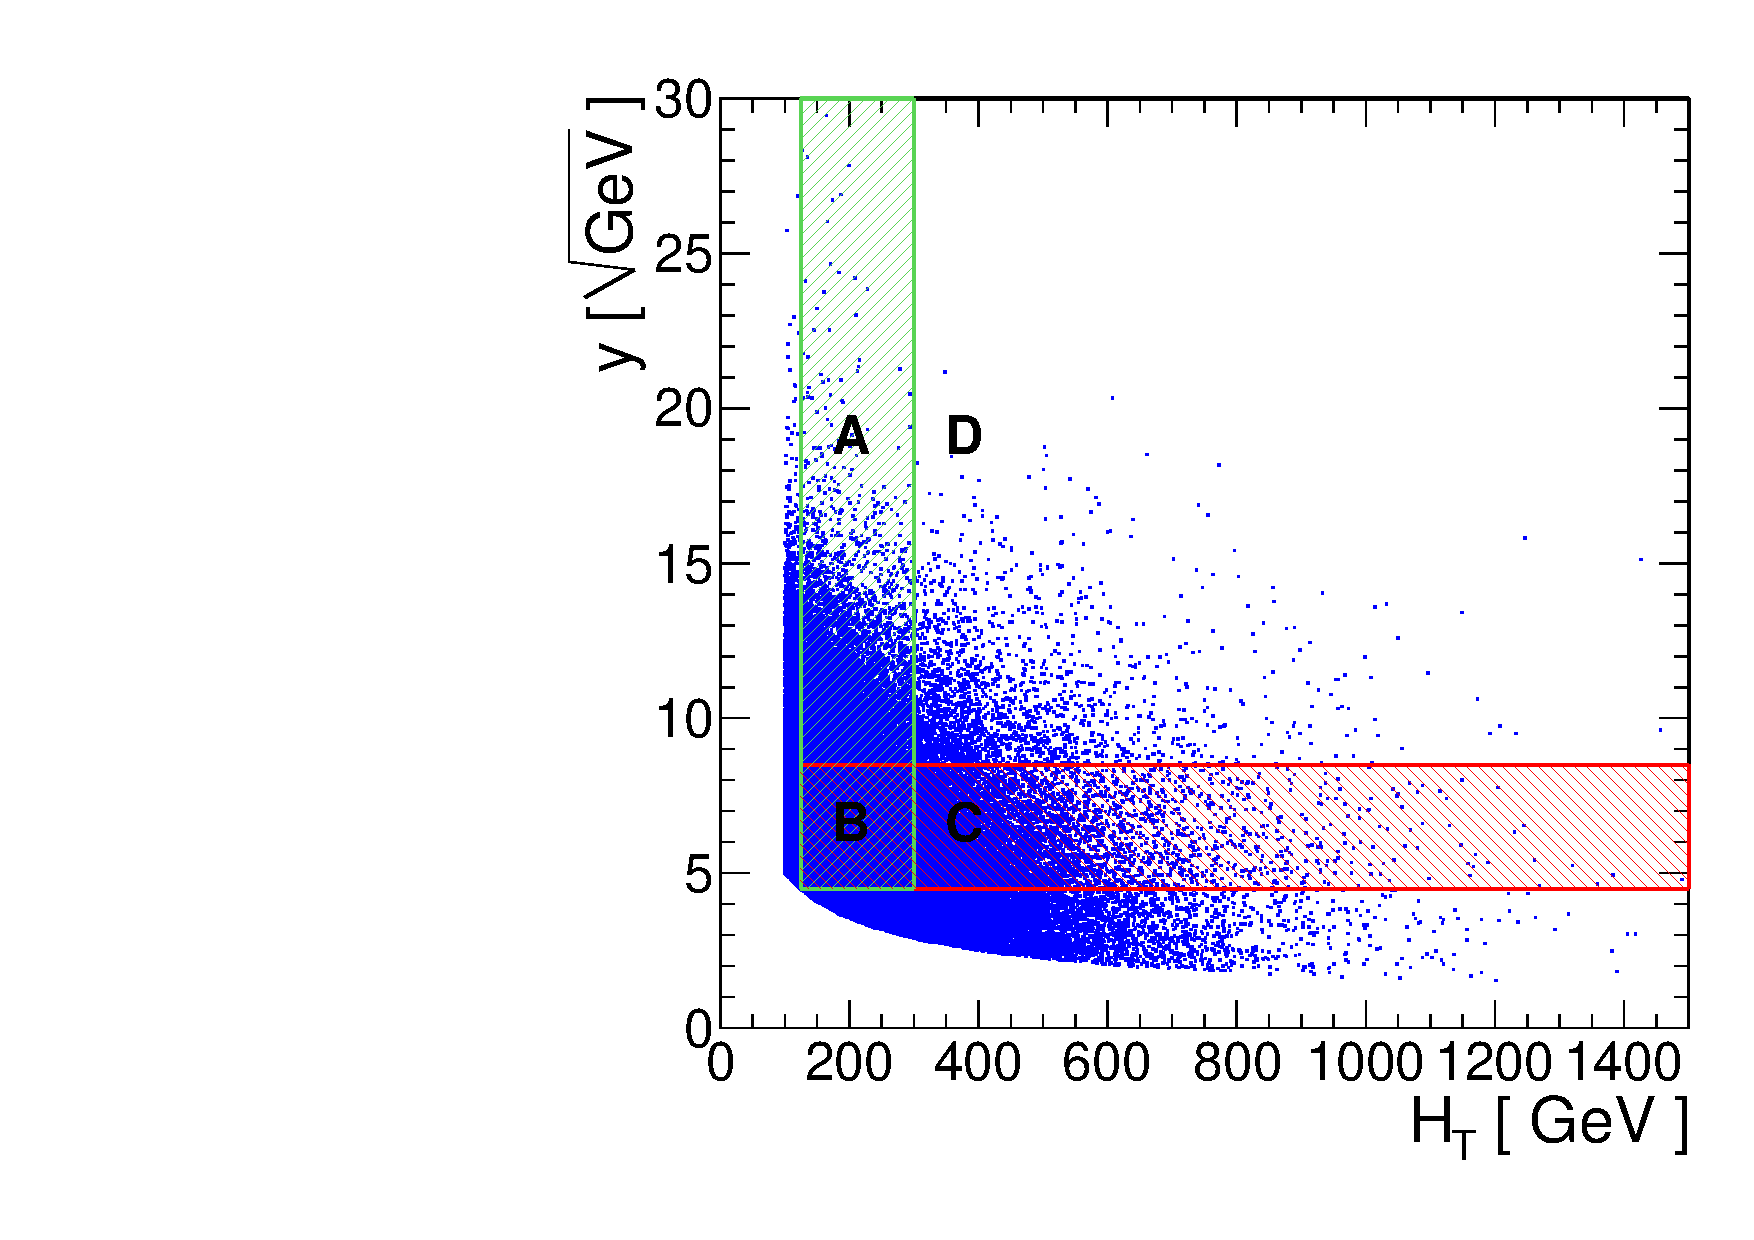
\includegraphics[width=0.6\linewidth]{plots/abcdprime.pdf}
\caption{\label{fig:abcdprime}\protect Distributions of $y$ 
vs. \Ht\ for \ttbar\ MC. The $f(y)$ and $g(H_T)$ functions are
measured using events in the green and red shaded areas, respectively.}
\end{center}
\end{figure}

\begin{figure}[tbh]
\begin{center}
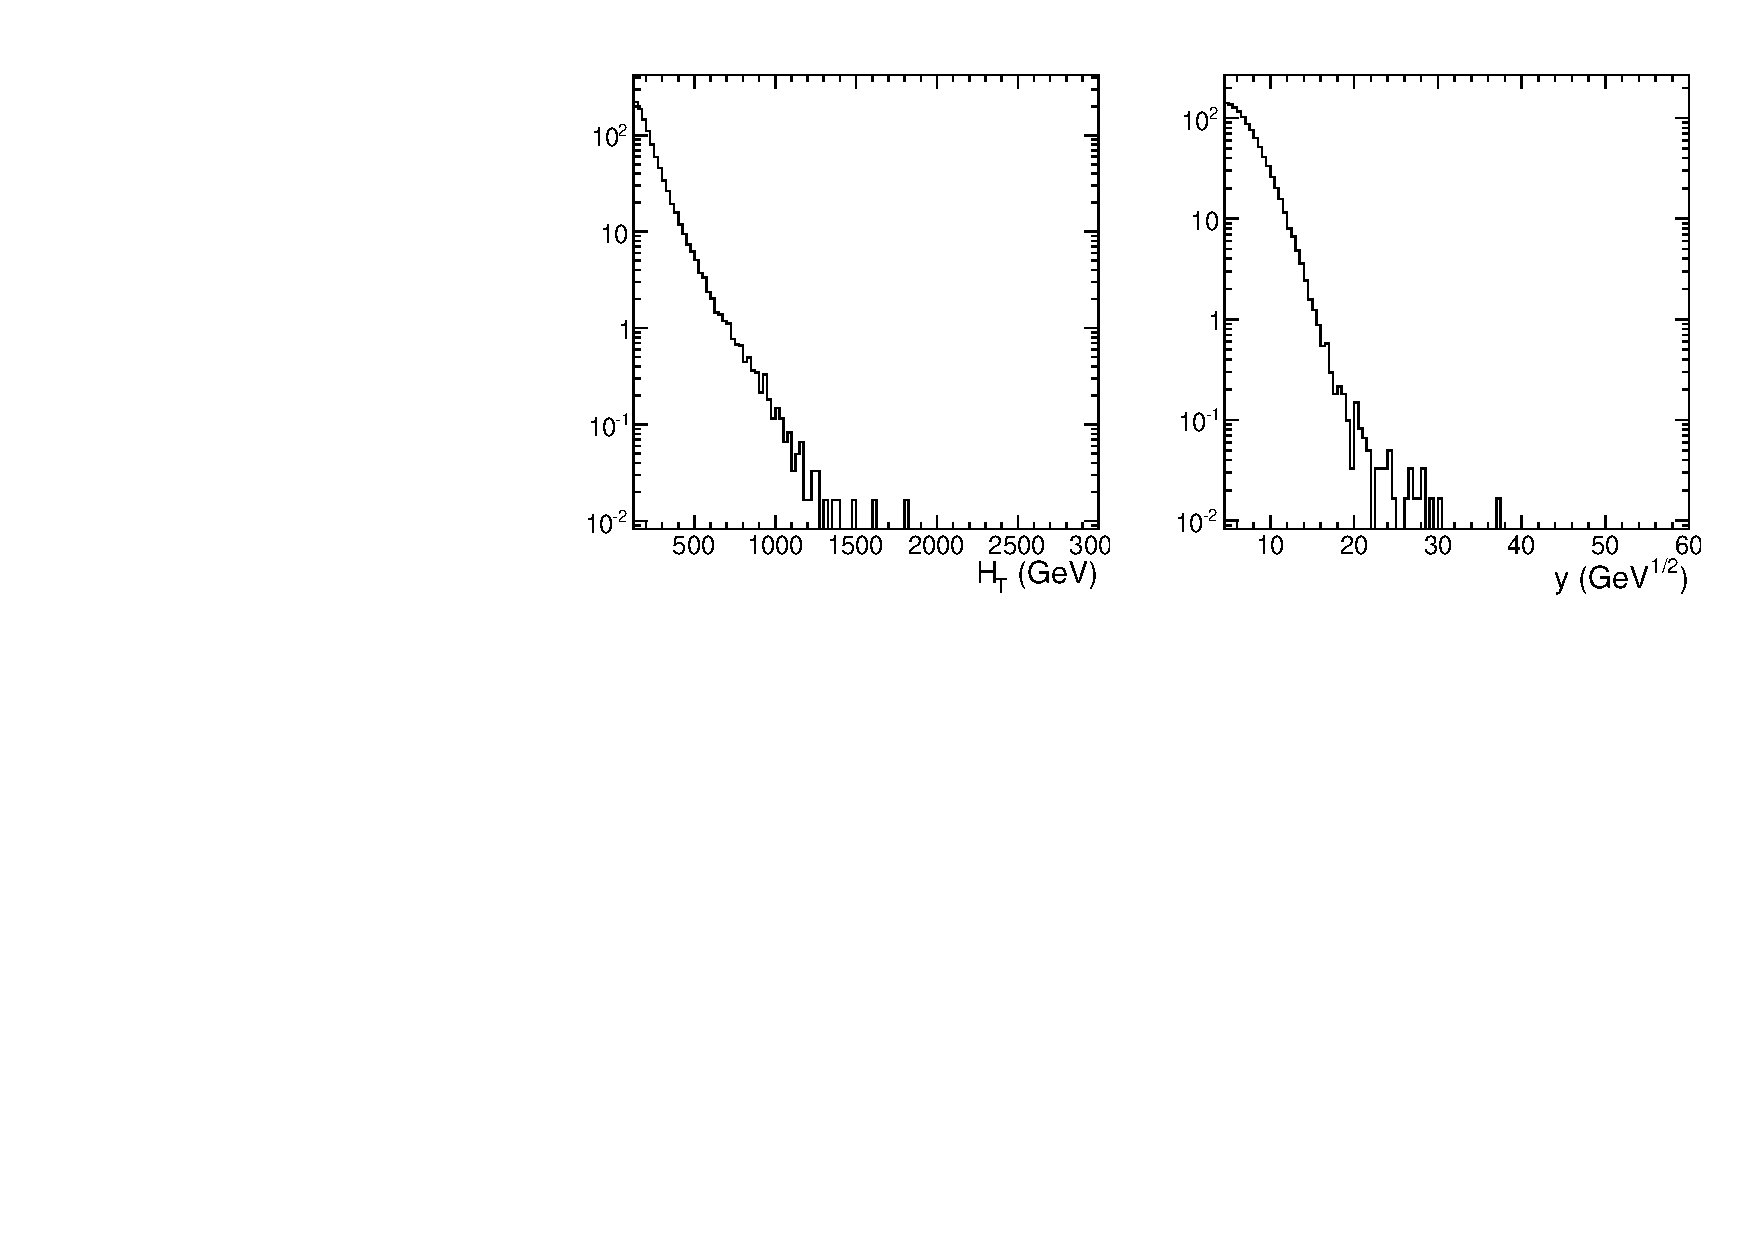
\includegraphics[width=1\linewidth]{plots/abcdprimedist.pdf}
\caption{\label{fig:abcddist}\protect The distributions $f(y)$ and $g(H_T)$ 
extracted from \ttbar\ MC.}
\end{center}
\end{figure}

In this section, we study the ABCD' technique by applying it to \ttbar\ MC (we use the powheg sample which has
10 times the number of dilepton events as the madgraph sample). As a cross-check,
we first use the ABCD' technique to estimate the background in the 2010 signal region
defined as $y > 8.5$~GeV$^{1/2}$ and \Ht\ $>$ 300~GeV, which may be compared to the 
prediction of the standard ABCD technique. We measure the $f(y)$ and $g(H_T)$ distributions
using events in the regions indicated in Fig.~\ref{fig:abcdprime}, yielding the
distributions shown in Fig.~\ref{fig:abcddist}. Next, we randomly sample values of $y$
and \Ht\ from these distributions; each pair of $y$ and \Ht\ values is a pseudo-event.
We generate 1 million pseudo-events, and find the ratio $R_{S/C}$, the ratio of the
number of pseudo-events falling in the 2010 signal region (ie. region D) to the number of pseudo-events
falling in a control region, defined as the OR of the A, B and C regions. We then
multiply this ratio by the number of \ttbar\ MC events which fall in the control region
to get the predicted yield, ie. $N_{pred} = R_{S/C} \times N({\rm control})$. 
To estimate the statistical uncertainty in the predicted background, we smear the bin contents
of $f(y)$ and $g(H_T)$ according to their uncertainties. We repeat the prediction 20 times
with these smeared distributions, and take the RMS of the deviation from the nominal prediction
as the statistical uncertainty. The results
are summarized in Table~\ref{tab:abcdprime2}, which show that the prediction of the
ABCD' method is consistent with that of the ABCD method within the statistical uncertainty.

We next apply the ABCD' technique to estimate the background in the regions:

\begin{itemize}
\item SR1: \met\ $>$ 275 GeV, \Ht\ $>$ 300 GeV
\item SR2: \met\ $>$ 200 GeV, \Ht\ $>$ 600 GeV. 
\end{itemize}

Note that we are unable to predict the yield in this region using
the standard ABCD technique, since \met\ and \Ht\ are not weakly correlated. The signal
regions are shown in Fig.~\ref{fig:abcdprime_met}. There is a sizable overlap between
SR2 and region C, hence when estimating the background for this signal region we
restrict the control region used to measure $g(H_T)$ and to determine  $N({\rm control})$ 
to $4.5 < y < 6.5$~GeV$^{1/2}$.
As summarized in Table~\ref{tab:abcdprime}, we find agreement between the observed and
predicted yields in these signal regions within $(30 \pm 10)$\% and $(5 \pm 7)$\% for SR1 and SR2, respectively. 

\begin{figure}[hbt]
\begin{center}
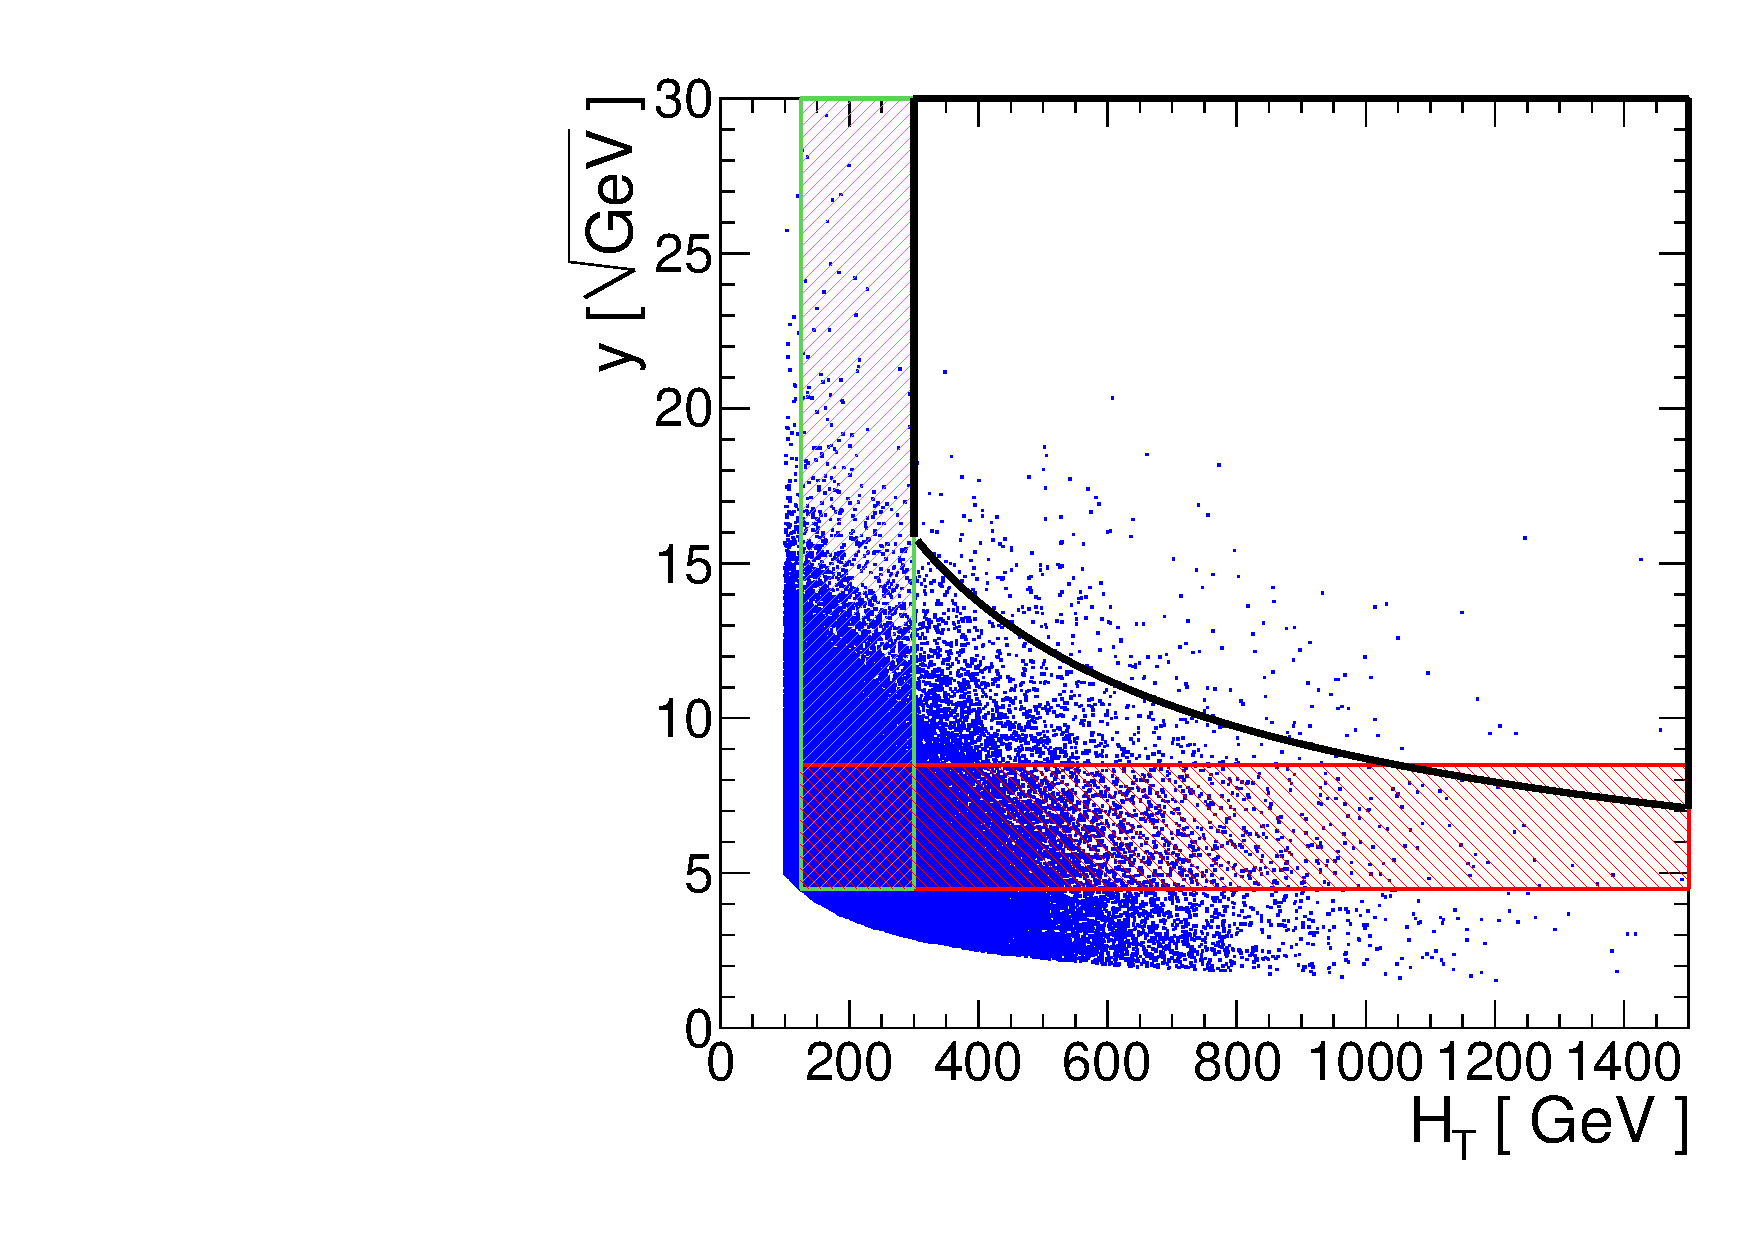
\includegraphics[width=0.48\linewidth]{plots/abcdprime_met275_ht300.pdf}
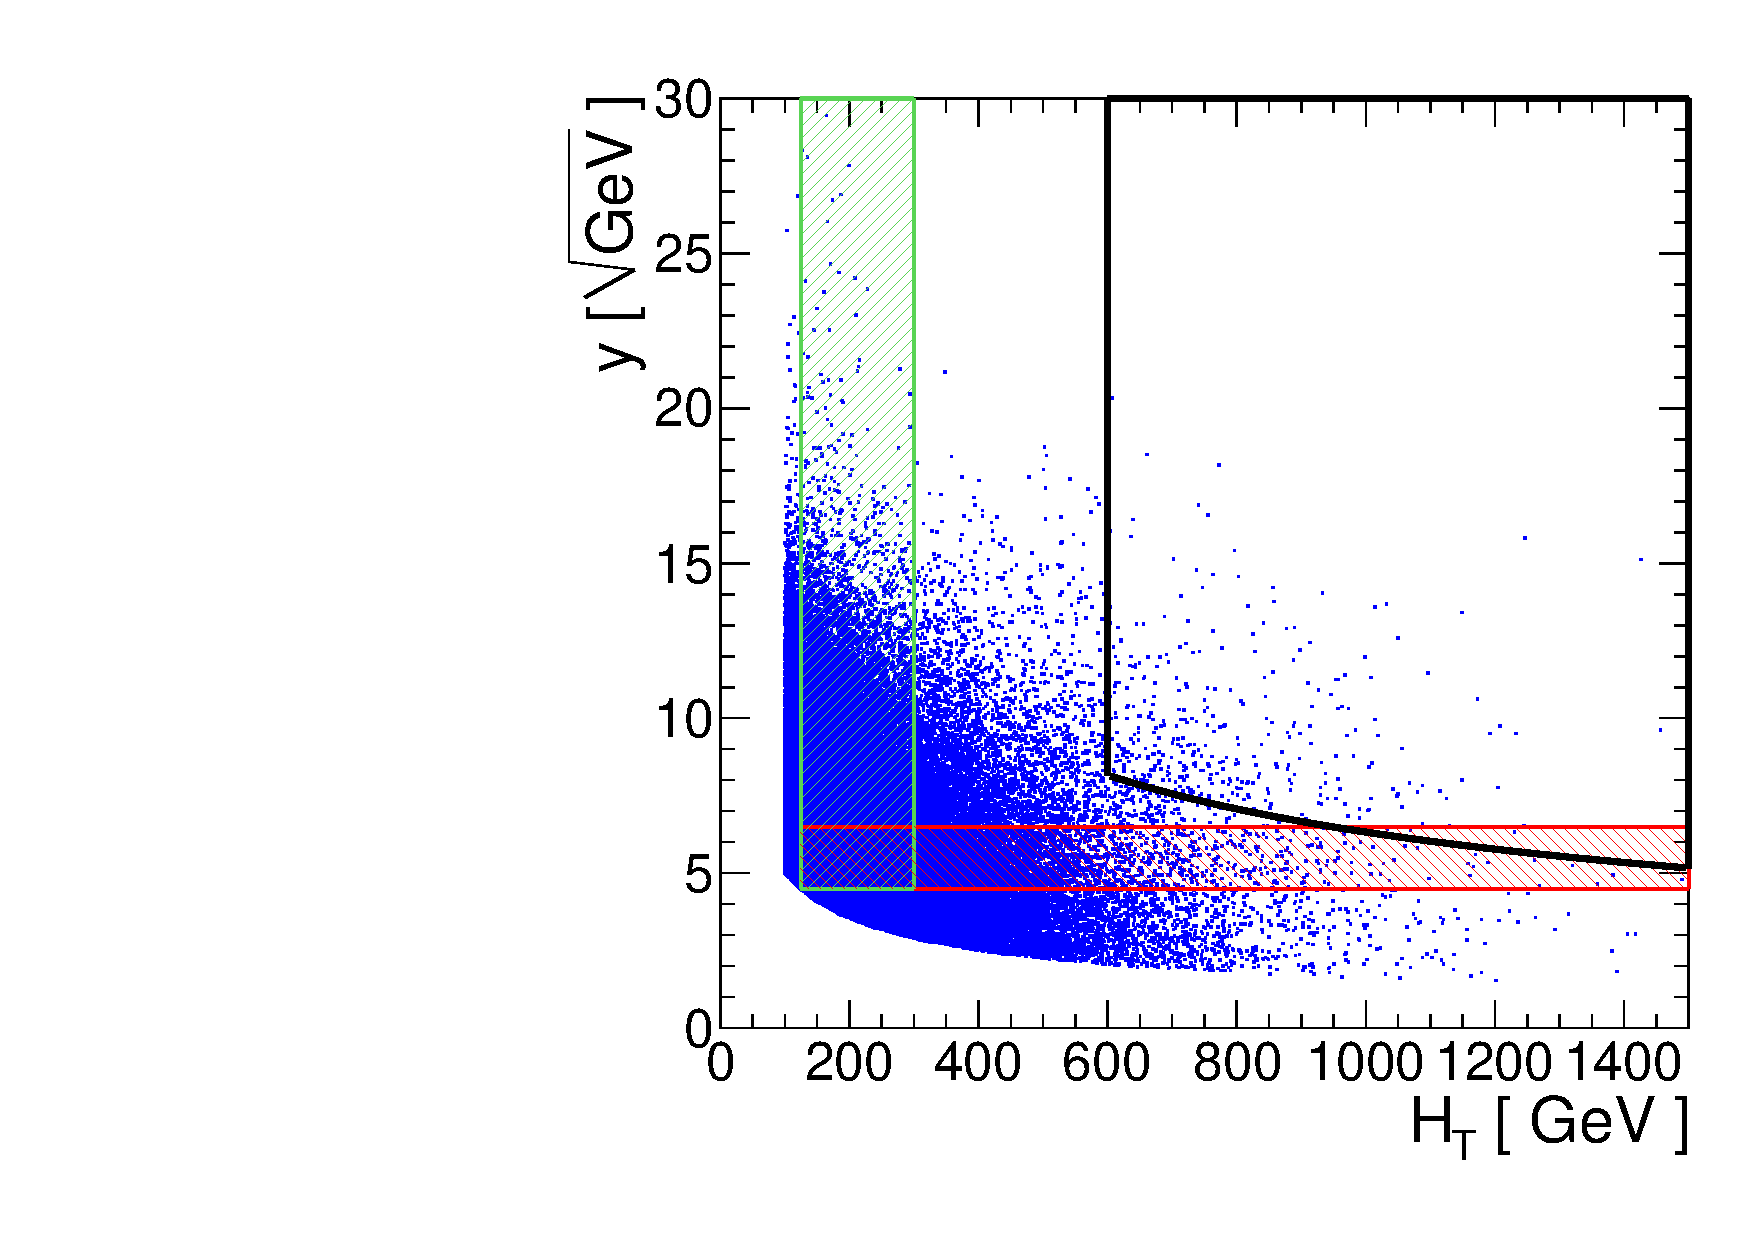
\includegraphics[width=0.48\linewidth]{plots/abcdprime_met200_ht600.pdf}
\caption{\label{fig:abcdprime_met}\protect 
Distributions of $y$ vs. \Ht\ for \ttbar\ MC. The signal regions \met\ $>$ 275 GeV, \Ht\ $>$ 300 GeV (left)
and \met\ $>$ 200 GeV, \Ht\ $>$ 600 GeV (right) are indicated with thick black lines. The $f(y)$ and $g(H_T)$ 
functions are measured using events in the green and red shaded areas, respectively.
}
\end{center}
\end{figure}


\begin{table}[hbt]
\begin{center}
\caption{\label{tab:abcdprime2} 
Summary of results expected results of the ABCD' method for 1 fb$^{-1}$ using \ttbar\ MC.
The quantities $R_{S/C}$ and $N({\rm control})$ are discussed in the text. The prediction of the 
ABCD' technique (ABCD' pred) is compared with the observed signal yield (observed) and 
where applicable, with the prediction of the ABCD technique (ABCD pred). The errors
in ABCD' pred and observed/ABCD' pred include only the statistical uncertainty in the
observed yield. 
}
\begin{tabular}{l|ccc}
\hline
                    &  2010 signal region         &    \met\ $>$ 275 GeV, \Ht\ $>$ 300 GeV & \met\ $>$ 200 GeV, \Ht\ $>$ 600 GeV \\
\hline                                                                                    
$R_{S/C}$            &       $3.5 \times 10^{-2}$   &          $2.8 \times 10^{-3}$           &     $4.9 \times 10^{-3}$         \\   
$N({\rm control})$  &       1239                  &             1239                       &      1187                        \\
ABCD' pred          &       43.4                  &              3.5 $\pm$ 0.1             &      5.9 $\pm$ 0.3               \\
observed            &       37.0 $\pm$ 0.8        &              4.5 $\pm$ 0.3             &      6.2 $\pm$ 0.3               \\
observed/ABCD' pred &       0.85 $\pm$ 0.02       &              1.30 $\pm$ 0.10           &      1.05 $\pm$ 0.07             \\                  
ABCD pred           &       43.0 $\pm$ 0.6        &              N/A                       &      N/A                         \\
\hline
\end{tabular}
\end{center}
\end{table}

{\bf WILL ADD HERE DESCRIPTION OF DEREK'S TOY STUDIES, AND DERIVE SYST UNCERTAINTIES BASED ON THEM}
